\documentclass[10pt,landscape]{exam}
\usepackage[phy]{template-for-exam}
\usepackage[margin=0.4in]{geometry}
\usepackage{multicol,silence,graphicx}

\WarningFilter{latex}{Label `question}
\WarningFilter{latex}{There were multiply-defined labels}
\WarningFilter{latex}{Label `part}
%%%%%%%%%%%%%%%%%%%%%%%%%%%%%%%%%%%%%

\def\todayDate{Mon, Feb 2}

\def\content{

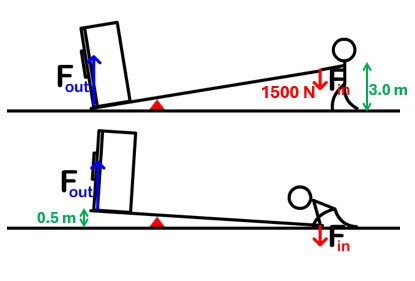
\includegraphics[width=3in]{lever.png}

\noindent
The man on the right side of the lever pushes the lever straight down 3.0~m.  He exerts a force of 1500~N.

\vspace{1em}

\begin{parts}
  \part Calculate the work done by the man. \vs
  \part The left side of the lever raises 0.5~m.  If the work done by the man is transferred to the left side, calculate the force on this side of the lever. \vs
  \part What mass of refrigerator could the man lift with this lever? \vs
\end{parts}

}

%%%%%%%%%%%%%%%%%%%%%%%%%%%%%%%%%%%%%%

\begin{document}
\pagestyle{empty}

\setlength{\columnsep}{0.8in}
\begin{multicols*}{2}

\noindent  
Name: \hfill Period: \hspace{5em}
\vspace{0.5em}
\hrule

\section*{\todayDate}
\subsection*{Warmup}

\content

\vfill
\hrule
\vspace{0.5em}
\hfill {\sc Physics I}

\columnbreak

\noindent  
Name: \hfill Period: \hspace{5em}
\vspace{0.5em}
\hrule

\section*{\todayDate}
\subsection*{Warmup}

\content

\vfill
\hrule
\vspace{0.5em}
\hfill {\sc Physics I}

\end{multicols*}

\end{document}